\documentclass{article}
\usepackage{graphicx} % Required for inserting images
\usepackage[english]{babel}
\usepackage{amsmath}
\usepackage{amsfonts}
\usepackage{amsthm}
\usepackage{amssymb}
\usepackage{physics}
\usepackage[mathscr]{euscript}
\let\euscr\mathscr \let\mathscr\relax
\usepackage[scr]{rsfso}
\newcommand{\powerset}{\raisebox{.15\baselineskip}{\Large\ensuremath{\wp}}}


\usepackage{mathtools}


\numberwithin{equation}{section}

\newcommand{\vbh}[1]{\vb{\hat{#1}}}
\newcommand{\set}[1]{\{#1\}}
\newcommand{\FT}{\mathcal{F}}
\newcommand\perm[2][^n]{\prescript{#1\mkern-2.5mu}{}P_{#2}}
\newcommand\comb[2][^n]{\prescript{#1\mkern-0.5mu}{}C_{#2}}

\DeclareMathOperator{\spn}{span}

\makeatletter
\renewcommand*\env@matrix[1][*\c@MaxMatrixCols c]{%
  \hskip -\arraycolsep
  \let\@ifnextchar\new@ifnextchar
  \array{#1}}
\makeatother

\newtheorem{theorem}{Theorem}[section]
\newtheorem{corollary}{Corollary}[theorem]
\newtheorem{lemma}[theorem]{Lemma}


\title{PHYS110A Homework 1}
\author{Siyu Chen}
\date{Summer 2023}

\begin{document}

\maketitle

\section{(1), (6), (11) vector identities on Griffith front cover.}

\paragraph{(1) $\vb{A \cdot (B \cross C) = B \cdot (C \cross A) = C \cdot (A \cross B)} \\$}

Consider $\vb{A \cdot (B \cross C)}$,

\begin{equation}
    \vb{A \cdot (B \cross C) = (A \cdot \hat{e}_k)} \epsilon_{ijk} b_i c_j = \epsilon_{ijk} b_i c_j a_k
\end{equation}

Now consider $\vb{B \cdot (C \cross A)}$

\begin{equation}
    \vb{B \cdot (C \cross A) = (B \cdot \hat{e}_k)} \epsilon_{ijk} c_i a_j = \epsilon_{ijk} c_i a_j b_k
\end{equation}

Lastly, let's consider $\vb{C \cdot (A \cross B)}$

\begin{equation}
    \vb{C \cdot (A \cross B) = (C \cdot \hat{e}_k)} \epsilon_{ijk} a_i b_j = \epsilon_{ijk} a_i b_j c_k
\end{equation}

Now, we can immediately see that, first, since all indices in the final expressions of our three equations appear twice, they will be summed over and therefore are dummy indices, and our final expression is a number, which is what we would expect since the cross product is a vector, and the dot product between two vectors will return a number. Next, from what we know from the Levi-Civita symbol, as it returns 0 if there is duplicates in the indices, and 1 for even permutations and -1 for odd permutations, we can see that in our final expressions, the parity of our permutation are the same as our dummy indices $i,j,k$ are cyclically arranged onto $a,b,c$ in such order. Therefore, we can see that the final expression for all three equations are the same, and therefore we have derived the result.

\paragraph{(6) $\vb{\grad \cdot (A \cross B) = B \cdot (\grad \cross A) - A \cdot (\grad \cross B)} \\$}

Consider LHS, we have 

\begin{equation}
    \begin{split}
        \vb{\grad \cdot (A \cross B)} &= \div \lbrack \epsilon_{ijk} a_i b_j \rbrack_k = \partial_k \lbrack \epsilon_{ijk} a_i b_j \rbrack_k \\
        &= \epsilon_{ijk} \partial_k (a_i) b_j + \epsilon_{ijk} \partial_k (b_j) a_i \\
        &= \epsilon_{ijk} \partial_k (a_i) \vb{B \cdot \hat{e}_j} + \epsilon_{ijk} \partial_k (b_j) \vb{A \cdot \hat{e}_i} \\
        &= \vb{B} \cdot \epsilon_{kij} \lbrack \partial_k a_i \rbrack_j - \vb{A} \cdot \epsilon_{kji} \lbrack \partial_k b_j \rbrack_i \\
        &= \vb{B \cdot (\curl A) - A \cdot (\curl B)}
    \end{split}
\end{equation}

Note: in (1.4), line 1, the implied summation of the index $k$ in the Levi-Civita symbol and the $k$ component of the bracket term sums to a vector as we iterate over $k$, which is why the divergence is a defined operator over it. In line 4, $\epsilon_{kij} = \epsilon_{ijk} = - \epsilon{kji}$ due to the properties of Levi-Civita symbol.

\paragraph{(11) $\vb{\curl (\curl A) = \grad (\div A) - \grad^2 A}$}

Consider LHS, we have

\begin{equation}
        \curl (\curl A) = \curl \epsilon_{ijk} \lbrack \partial_i a_j \rbrack_k = \epsilon_{lkm} \epsilon_{ijk}  \lbrack \partial_l (\partial_i a_j)_k \rbrack_m  
\end{equation}

Evaluating the product of the two Levi-Civita symbols, we have:

\begin{equation}
    \begin{split}
        \epsilon_{lkm} \epsilon_{ijk} = \begin{vmatrix}
            \delta_{li} & \delta_{lj} & \delta_{lk} \\ \delta_{ki} & \delta_{kj} & \delta_{kk} \\ \delta_{mi} & \delta_{mj} & \delta_{mk} 
        \end{vmatrix} = \delta_{mi} \delta_{lj} - \delta_{li} \delta_{mj} 
    \end{split}
\end{equation}

Going back to (1.5), we have

\begin{equation}
    \begin{split}
        \text{LHS} &=  (\delta_{mi} \delta_{lj} - \delta_{li} \delta_{mj} ) \lbrack \partial_l (\partial_i a_j)_k \rbrack_m \\
        &= \delta_{mi} \delta_{lj} \lbrack \partial_l (\partial_i a_j)_k \rbrack_m - \delta_{li} \delta_{mj} \lbrack \partial_l (\partial_i a_j)_k \rbrack_m \\
        &= \lbrack \partial_j (\partial_i a_j)_k \rbrack_i -  \lbrack \partial_i (\partial_i a_j)_k \rbrack_j \\
        &=  (\partial_j \partial_i a_j \vb{\hat{e}_i) \hat{e}_k} -  (\partial_i \partial_i a_j \vb{\hat{e}_j}) \vb{\hat{e}_k} \\
        &= \partial_i \vb{\hat{e}_i (\div A) \hat{e}_k - \grad^2 A \hat{e}_k} \\ 
        &= \vb{\grad (\div A) - \grad^2 A}
    \end{split}
\end{equation}

Note: in (1.7), line 3, since the only way that the product of two deltas would be 1 is that both delta would return 1, therefore both pairs of indices on both of the deltas would have to be the same, i.e $m = i, l = j$ and $l = i, m = j$, respectively. In line 4, we simply group the similar indices of $i, j$ to sum them over; since the expression in the brackets are scalars, the scalar multiplication over $\vb{\hat{e}_k}$ is justified. Lastly, we iterate over $k$ to obtain our full vectors.

\section{Problem 1.9}

\paragraph{Find the transformation matrix R that describes a rotation by $120^\circ$ about an axis from the origin through the point $(1, 1, 1)$. The rotation is clockwise as you look down the axis toward the origin. \\}

As we look down the axis toward the origin, we can see that the three axis form a three-fold rotational symmetry about the line between $(1,1,1)$ and the origin. We can use the rotational transformation formula, or we can realize, that with the three-fold rotational symmetry that this shape forms, and with a rotation of $120^\circ$, which is one-third of a full rotation, we would just be changing the permutation of our axis. Since our rotation is clockwise, and assuming that we structure our axis according to the Right Hand Rule, $x$-axis would transform to the new $z$-axis, $y$-axis the new $x$-axis and $z$-axis the new $y$-axis. Therefore the matrix for such transformation is given by:

\begin{equation}
    R = \begin{pmatrix}
        0 & 1 & 0 \\ 0 & 0 & 1 \\ 1 & 0 & 0
    \end{pmatrix}
\end{equation}

\begin{figure}[!htb]
    \centering
   \begin{minipage}{0.48\textwidth}
     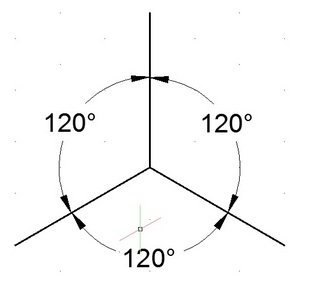
\includegraphics[width=.7\linewidth]{hw/hw1/2.1.jpg}
     \caption{The three-fold rotational symmetry shape formed by original axis as seen from rotational axis. Image from internet.}\label{Fig: 2.1}
   \end{minipage}
\end{figure}

\section{Problem 1.13}

\textbf{Let $\vb{r}$ be the separation vector from a fixed point $(x',y',z')$ to the point $(x,y,z)$, and let $r $ be its length. Show that}

\paragraph{(a) $\grad^2 (r^2) = 2 \vb{r}$ \\}

We know that $r = \sqrt{(x-x')^2 + (y-y')^2 + (z-z')^2}$, consider LHS,

\begin{equation}
\begin{split}
    \grad r^2 &= \grad ((x-x')^2 + (y-y')^2 + (z-z')^2) \\
    &= 2(x-x') \vb{\hat{x}} + 2(y-y') \vb{\hat{y}} + 2(z-z') \vb{\hat{z}} = 2 \vb{r}
\end{split}
\end{equation}

\paragraph{(b) $\grad(\frac{1}{r}) = - \frac{\vb{\hat{r}}}{r^2}$\\}

Consider LHS:

\begin{equation}
\begin{split}
    \grad(\frac{1}{r}) &= \grad (\frac{1}{((x-x')^2 + (y-y')^2 + (z-z')^2)^\frac{1}{2}}) \\
    &= -\frac{1}{2}\frac{1}{r^3} ( 2(x-x') \vb{\hat{x}} + 2(y-y') \vb{\hat{y}} + 2(z-z') \vb{\hat{z}} \\
    &= - \frac{1}{r^3} \vb{r} = - \frac{\vb{\hat{r}}}{r^2}
    \end{split}
\end{equation}

\paragraph{(c) What is the general formula for $\grad(r^n)$?\\}

We can see that $r^n = ((x-x')^2 + (y-y')^2 + (z-z')^2)^\frac{n}{2}$. Now consider $\grad (r^n)$:

\begin{equation}
    \begin{split}
        \grad (r^n) &= \grad ((x-x')^2 + (y-y')^2 + (z-z')^2)^\frac{n}{2} \\
        &= \frac{n}{2} ((x-x')^2 + (y-y')^2 + (z-z')^2)^{\frac{n-2}{2}} 2 \vb{r} \\
        &= nr^{n-2} 2\vb{r} = 2n r^{n-1} \vb{\hat{r}}
    \end{split}
\end{equation}

\section{Problem 1.17}

\paragraph{In two dimensions, show that the divergence transforms as a scalar
under rotations.\\}

Let $\vb{v} = v_x \vb{\hat{x}} + v_y \vb{\hat{y}}$ be a vector in 2-D. Let $R$ be the matrix of a counter-clockwise rotational transformation in 2-D by $\phi$. Let $\overline{\vb{v}} = R \vb{v} = (v_x \cos \phi + v_y \sin \phi) \vb{\hat{x}} + (- v_x \sin \phi + v_y \cos \phi) \vb{\hat{y}}$ We have to show the following:

\begin{equation}
    \vb{\div v = \div \overline{v}}
\end{equation}

Consider the LHS, it is clear that it is just $\partial_x v_x + \partial_y v_y$. Now consider the RHS:

\begin{equation}
\begin{split}
    \text{RHS} &= \partial_{\overline{x}} \overline{v_x} + \partial_{\overline{y}}  \overline{v_y} \\
    &= \partial_x (v_x \cos \phi + v_y\sin \phi) \frac{\partial x}{\partial \overline{x}} + \partial_y  (-v_x\sin \phi + v_y\cos \phi) \frac{\partial y}{\partial \overline{y}}
\end{split}
\end{equation}

Let's consider $\frac{\partial x}{\partial \overline{x}}, \frac{\partial y}{\partial \overline{y}}$:

\begin{equation}
\begin{split}
\overline{x} &= x \cos \phi + y \sin \phi \\
x &= \frac{\overline{x}}{\cos \phi} - \frac{y \sin \phi}{\cos \phi} \\
    \frac{\partial x}{\partial \overline{x}} &=  \frac{1}{\cos \phi}
    \end{split}
\end{equation}

and respectively:

\begin{equation}
\begin{split}
    \overline{y} &= -x \sin \phi + y \cos \phi \\
    y &= \frac{\overline{y}}{\cos \phi} + \frac{x \sin \phi}{\cos \phi}\\
    \frac{\partial y}{\partial \overline{y}} &= \frac{1}{\cos \phi}
    \end{split}
\end{equation}

Going back to (4.2), it becomes:

\begin{equation}
    \text{RHS} = \partial_x v_x + \partial_x v_y \tan \phi - \partial_y v_x \tan \phi + \partial_y v_y = \partial_x v_x + \partial_y v_y = \text{LHS}
\end{equation}

since the mismatched derivatives return $0$

\section{Problem 1.25}

\paragraph{(a) Check product rule (iv) (by calculating each term separately) for the functions: \\}

\begin{equation*}
    \vb{A} = x \vb{\hat{x}} + 2y \vbh{y} + 3z \vbh{z}; \quad \vb{B} = 3y \vbh{x} - 2x \vbh{y}
\end{equation*}

Just for utility, let's compute some useful quantities:

\begin{equation}
    \begin{split}
        \vb{A \cross B} &= 6xz \vbh{x} + 9yz \vbh{y} + (- 2x^2 - 6y^2) \vbh{z} \\
        \vb{A \cdot B} &= 3xy - 4xy = -xy \\
        \vb{\curl A} &= 0, \quad \vb{\curl B} = -5 \vbh{z} \\
        \vb{\div A} &= 6, \quad \vb{\div B} = 0
    \end{split}
\end{equation}

We have to verify that:

\begin{equation}
    \vb{\div (A \cross B) = B \cdot (\curl A) - A \cdot (\curl B) }
\end{equation}

Let's consider LHS first:

\begin{equation}
    \text{LHS} = \div (6xz \vbh{x} + 9yz \vbh{y} + (- 2x^2 - 6y^2) \vbh{z}) = 6z  + 9z = 15z
\end{equation}

Then let's compute RHS:

\begin{equation}
    \text{RHS} = B \cdot (\vb{0}) - A \cdot (-5 \vbh{z}) = 5\cdot3z = 15 z = \text{LHS}
\end{equation}

\paragraph{(b) Do the same for product rule (ii).\\}

We have to verify:

\begin{equation}
    \vb{\grad (A \cdot B) = A \cross (\curl B) + B \cross (\curl A) + (A \cdot \grad) B + (B \cdot \grad) A}
\end{equation}

let's compute LHS first:

\begin{equation}
    \text{LHS} = \grad (-xy) = - y \vbh{x} - x \vbh{y}
\end{equation}

let's compute RHS next:

\begin{equation}
    \begin{split}
        \text{RHS} &= -5 \vb{A \cross \hat{z}} + 0 + (x \partial_x + 2y \partial_y + 3z \partial_z) \vb{B} + (3y \partial_x - 2x \partial_y) \vb{A} \\
        &= -5 \vb{A} \cross \vbh{z} + 0 + -2 x \vbh{y} + 6y\vbh{x} + 3y\vbh{x} - 4x \vbh{y} \\
        &= -10 y \vbh{x} + 5x \vbh{y} - 6x \vbh{y} + 9 y \vbh{x} = - y \vbh{x} - x \vbh{y} = \text{LHS}
    \end{split}
\end{equation}

\paragraph{(c) Do the same for product rule (vi).\\}

We have to verify:

\begin{equation}
    \vb{ \curl ( A \cross B) = (B \cdot \grad) A - (A \cdot \grad) B + A (\grad \cdot B) - B (\grad \cdot A)}
\end{equation}

Let's compute LHS first:

\begin{equation}
    \text{LHS} = \curl (6xz \vbh{x} + 9zy \vbh{y} + (-2x^2 - 6y^2) \vbh{z}) = -21 y\vbh{x} + 10 x \vbh{y}
\end{equation}

Then let's compute RHS, we can find the first two terms from part (b)

\begin{equation}
\begin{split}
    \text{RHS} &= 3y \vbh{x} - 4x \vbh{y} + 2x\vbh{y} - 6y \vbh{x} + 0 - 6\vb{B} \\
    &= -3y \vbh{x} - 2x \vbh{y} - 18 y\vbh{x} + 12 x \vbh{y} = -21 y\vbh{x} + 10 x \vbh{y} = \text{LHS}
    \end{split}
\end{equation}

\section{Problem 1.29}

\textbf{Calculate the line integral of the function $\vb{v} = x^2 \vbh{x} + 2yz \vbh{y} + y^2 \vbh{z}$ from the origin to the point $(1,1,1)$ by three different routes:}
\paragraph{(a) (0, 0, 0) → (1, 0, 0) → (1, 1, 0) → (1, 1, 1).\\}

The line integral can be written as:

\begin{equation}
\begin{split}
    \int_{C} \vb{v} \cdot d \vb{r} &= \int_{(0,0,0)}^{(1,0,0)} v_x dx + \int_{(1,0,0)}^{(1,1,0)} v_y dy + \int_{(1,1,0)}^{(1,1,1)} v_z dz \\
    &= \frac{1}{3} x^3 \rvert^{1}_{0} + y^2z \rvert^{(1,1,0)}_{(1,0,0)} + y^2z \rvert^{(1,1,1)}_{(1,1,0)} \\ 
    &= \frac{1}{3} + 0 + 1 = \frac{4}{3}
    \end{split}
\end{equation}

\paragraph{(b) (0, 0, 0) → (0, 0, 1) → (0, 1, 1) → (1, 1, 1).\\}

\begin{equation}
\begin{split}
    \int_{C} \vb{v} \cdot d \vb{r} &= \int_{(0,0,0)}^{(0,0,1)} v_z dz + \int_{(0,0,1)}^{(0,1,1)} v_y dy + \int_{(0,1,1)}^{(1,1,1)} v_x dx \\
    &= \frac{1}{2} y^2 z^2 \rvert^{(0,0,1)}_{(0,0,0)} + y^2z \rvert^{(0,1,1)}_{(0,0,1)} + x^3 \rvert^{(1,1,1)}_{(0,1,1)} \\ 
    &= 0+ 1 + \frac{1}{3} = \frac{4}{3}
    \end{split}
\end{equation}

\paragraph{(c) The direct straight line.\\}

Let $\vb{t} = t (\vbh{x}+\vbh{y}+\vbh{z}) \quad 0 \leq t \leq 2$ and $t = x = y = z$

\begin{equation}
    \int_{C} \vb{v} \cdot d \vb{r} = \int_{0}^{1} \vb{v \cdot \vb{t}} dt = \int_0^1 t^2 + 2t^2 + t^2 dt = \frac{4}{3} t^3 \rvert^1_0 = \frac{4}{3}
\end{equation}

\paragraph{(d) What is the line integral around the closed loop that goes out along path (a) and back along path (b)? \\}

Since the curl of $\vb{v}$ is 0, it is a conservative vector field, therefore around any close loop, the line integral is 0.

\section{Problem 1.39}

\paragraph{(a) Check the divergence theorem for the function $\vb{v_1} = r^2 \vbh{r}$, using as your volume the sphere of radius $R$, centered at the origin.\\}

The divergence theorem states that:

\begin{equation}
    \int_{V} (\grad \cdot \vb{F}) dV = \int_{\partial V} \vb{F} \cdot d \vb{a}
\end{equation}

Let's evaluate LHS first:

\begin{equation}
    \text{LHS} = \int_V r^{-2} \partial_r r^4 dV = \int_V 4 r dV = \int^R_0 dr 4r^3 \int_0^{2\pi} d \phi \int^\pi_0 \sin \theta d \theta = 4 \pi R^4
\end{equation}

Let's evaluate RHS next, $R$ is constant on the surface

\begin{equation}
    \text{RHS} = \int_{\partial V} R^2 \sin \theta d\theta d\phi = R^4 \int_{0}^{2\pi} d \phi \int_{0}^\pi \sin \theta d \theta = 4 \pi R^4
\end{equation}

\paragraph{(b) Do the same for $\vb{v_2} = \frac{1}{r^2} \vbh{r}$\\}

Let's evaluate LHS first:

\begin{equation}
    \text{LHS} = \int_V (\div \vb{v_2}) dV = \int_V r^{-2} (\partial_r 1) dV = 0
\end{equation}

Note, for this case, the divergence is not defined at $r = 0$ for $\vb{v_2} = \frac{1}{r^2}$. Let's compute RHS next, where $R$ is constant at the surface

\begin{equation}
    \text{RHS} = \int_{\partial V} \frac{1}{R^2} d \vb{a} =\int_{0}^\pi \int_0^{2\pi} R^2 \frac{1}{R^2} \sin \theta d \theta d \phi = 4 \pi
\end{equation}

The difference is due to the discontinuity at $r = 0$ for the first method. 

\section{Problem 1.40}

\textbf{Compute the divergence of the function}
\begin{equation*}
    \vb{v} = (r \cos \theta) \vbh{r} + (r \sin \theta) \vbh{\theta} + (r \sin \theta \cos \phi) \vbh{\phi}
\end{equation*}
\paragraph{Check the divergence theorem for this function, using as your volume the inverted hemispherical bowl of radius $R$, resting on the $xy$ plane and centered at the origin. \\}

Let's compute the divergence of our function first:

\begin{equation}
\begin{split}
    \div \vb{v} &= r^{-2} \partial_r (r^3 \cos \theta) + r^{-1} \sin^{-1} \theta \partial_\theta (r \sin^2 \theta ) + r^{-1} \sin^{-1}\theta \partial_\phi ( r \sin \theta \cos \phi) \\
    &= 3 \cos \theta + 2 \cos \theta - \sin \phi = 5 \cos \theta - \sin \phi
\end{split}
\end{equation}

Let's evaluate the LHS, volume integral, of the divergence theorem first:

\begin{equation}
\begin{split}
    \int_V \div \vb{v} dV &= \int_0^R \int_0^{2\pi} \int_0^{\frac{\pi}{2}}  r^2 \sin \theta (5\cos \theta - \sin \phi) dr d \theta d \phi \\
    &= \frac{1}{3} R^3 \int_0^{2\pi} d\phi \int_0^{\pi/2} d \theta ( 5\sin \theta \cos \theta - \sin \theta \sin \phi ) \\
    &= \frac{10\pi}{3} R^3 \int_0^{\frac{\pi}{2}} d \theta (\sin \theta \cos \theta) = \frac{5\pi}{3} R^3 
    \end{split}
\end{equation}

Let's evaluate the RHS, the surface integral side, of the divergence theorem next. Notice that we have to evaluate two surfaces, the hemisphere and the bottom:

\begin{equation}
    \begin{split}
        \int_{\partial V} \vb{v} \cdot d\vb{a} &= \int_{\text{hemisphere}} \ldots + \int_{\text{bottom}} \ldots
    \end{split}
\end{equation}

Evaluating the hemiphere side, the radius is constant at $R$.

\begin{equation}
    \int_{\text{hemisphere}} \ldots = \int_{S} r^3 \cos \theta d\vb{a} = \int_{0}^{\pi/2} d\theta \int_{0}^{2\pi} d\phi (R^3 \sin \theta \cos \theta) = \pi R^3
\end{equation}

Evaluating the bottom side, $d \vb{a} = r dr d\phi \vbh{\theta}$, $\theta = \pi/2, sin \theta = 1$

\begin{equation}
    \int_{\text{bottom}} \ldots = \int_S r \sin \theta d \vb{a} = \int_0^{2\pi} d\phi \int_0^{R} r^2 = \frac{2 \pi }{3} R^3  
\end{equation}

Combining the two terms, we finally have:

\begin{equation}
    \text{RHS} = \int_{\partial V} \vb{v} \cdot d \vb{a} = \pi R^3 + \frac{2}{3} \pi R^3 = \frac{5\pi}{2} R^3 = \text{LHS}
\end{equation}

and we have verified the Divergence Theorem for this function.

\section{Problem 1.49}

\textbf{Evaluate the integral}

\begin{equation*}
    J = \int_{\nu} e^{-r} (\div \frac{\vbh{r}}{r^2}) d \tau
\end{equation*}

\paragraph{(where $\nu$ is a sphere of radius $R$, centered at the origin) by two different methods:\\}

Using the first method, we have: 

\begin{equation}
    J = \int_{\nu} e^{-r} 4 \pi \delta^3 (\vb{r}) d \tau = e^0 4 \pi = 4 \pi 
\end{equation}

Using the second method, we have 

\begin{equation}
    J = - \int_\nu \frac{\vbh{r}}{r^2} \cdot \lbrack \grad e^{-r} \rbrack d \tau + \oint_{\partial \nu} e^{-r} \frac{\vbh{r}}{r^2} \cdot d \vb{a}
\end{equation}

the gradient is:

\begin{equation}
    \grad e^{-r} = \frac{\partial e^{-r}}{\partial r} \grad r = -e^{-r} \vbh{r} + \oint_{\partial \nu} e^{-r} \frac{\vbh{r}}{r^2} \cdot d \vb{a}
\end{equation}

our integral therefore becomes:

\begin{equation}
    J = \int_{\nu} e^{-r} \frac{1}{r^2} d\tau + \oint_{\partial \nu} e^{-r} \frac{\vbh{r}}{r^2} \cdot d \vb{a} 
\end{equation}

Evaluating the first integral, we have:

\begin{equation}
    \int_0^R dr \int_0^{2\pi} d \phi \int_0^{\pi/2} d \theta (e^{-r} \sin \theta) = 4\pi (1-e^{-R}) 
\end{equation}

evaluating the second integral, we have:

\begin{equation}
    \oint_{\partial \nu} e^{-r} \frac{\vbh{r}}{r^2} \cdot d \vb{a} = \int_0^{\pi/2} d \theta \int_0^{2\pi} d \phi e^{-R} \sin \theta = 4 \pi e^{-R}
\end{equation}

combining the two terms, we have:

\begin{equation}
    J = 4 \pi (1 - e^{-R}) + 4 \pi e^{-R} = 4\pi 
\end{equation}

\section{Problem 1.61}

\textbf{Although the gradient, divergence, and curl theorems are the fundamental integral theorems of vector calculus, it is possible to derive a number of corollaries from them. Show that:}

\paragraph{(a) $\int_\nu (\grad T) d \tau = \oint_S T d \vb{a}$ \\}

Let $\vb{v = c}T$ where $\vb{c}$ is constant vector. Consider the Divergence Theorem for such a $\vb{v}$:

\begin{equation}
\begin{split}
    \int_\nu (\grad \vb{v}) d \tau &= \oint_S \vb{v} d \vb{a} \\
    \int_\nu \div (T \vb{c})  d \tau &= \oint_S (T \vb{c}) \cdot d \vb{a}
    \end{split}
\end{equation}

Using the product rule, we have:

\begin{equation}
    \begin{split}
        \int_\nu \div \vb{c} T d \tau + \int_\nu (\grad T) \cdot \vb{c} d \tau &= \oint_S (T \vb{c}) \cdot d \vb{a} 
    \end{split}
\end{equation}

Since $\vb{c}$ is a constant vector, therefore its gradient is $0$. We have 

\begin{equation}
     \int_\nu (\grad T) \cdot \vb{c} d \tau = \oint_S (T \vb{c}) \cdot d \vb{a}
\end{equation}

Since $\vb{c}$ is a constant vector, we can write it as $\vb{c} = c \vbh{c}$. Obviously, we can take $c$ the constant scalar out of the integral, but we can also take the $\vbh{c}$, our arbitrary unit vector direction out of the integral, since it does not matter whether we choose the direction of our vector before or after the integral. Therefore, our integral becomes:

\begin{equation}
    c \vbh{c} \cdot \int_\nu (\grad T) d \tau = c \vbh{c} \cdot \oint_S T d \vb{a}
\end{equation}

The constants cancel, and since this equation holds for any arbitrary direction of $\vbh{c}$, we can conclude that:

\begin{equation}
    \int_\nu (\grad T) d \tau =\oint_S T d \vb{a}
\end{equation}

\paragraph{(b) $\int_\nu (\curl \vb{v}) d \tau = - \oint_S \vb{v} \cross d \vb{a}$ \\}

Consider the Divergence Theorem for $(\vb{v \cross c)}$ where $\vb{c}$ is a constant vector.
\begin{equation}
    \int_\nu \div (\vb{v \cross c}) d \tau =\oint_S (\vb{v \cross c}) \cdot d \vb{a}
\end{equation}

Using product rule, and since the curl of $\vb{c}$ is 0, we can rewrite the LHS part inside the integral as

\begin{equation}
    \div (\vb{v \cross c}) = \vb{c \cdot (\curl v) - v \cdot (\curl c)} = \vb{c \cdot (\curl v) }
\end{equation}

We can rewrite the integral on RHS with the cross product anti-communicative property and the scalar triple product property that since it is describing a volume formed by the three vectors, that switching the order of operation while maintaining the same permutation does not change the outcome.

\begin{equation}
    \oint_S (\vb{v \cross c}) \cdot d \vb{a} = - \oint_S (\vb{c \cross v}) \cdot d \vb{a} = - \oint_S (\vb{c \cdot v}) \cross d \vb{a}
\end{equation}

we can put together our original integral as:

\begin{equation}
    \int_\nu \vb{c \cdot (\curl v)} d \tau = -  \oint_S (\vb{c \cdot v}) \cross d \vb{a}
\end{equation}

taking out the constant vector $\vb{c}$ of the integral by the same logic as part (a) and we obtain our desired expression:

\begin{equation}
    \int_\nu \vb{\curl v} d \tau= -  \oint_S \vb{v} \cross d \vb{a}
\end{equation}

\paragraph{(c) $\int_\nu (T \grad^2 U + (\grad T) \cdot (\grad U) d \tau = \oint_S (T \grad U) \cdot d\vb{a}$ \\}

Let $\vb{v} = T \grad U$, consider the Divergence Theorem for $\vb{v}$

\begin{equation}
    \int_\nu \div (T \grad U) d \tau =\oint_S (T \grad U) \cdot d \vb{a}
\end{equation}

Our RHS is the same as our desired expression, let's consider inside of LHS and apply product rule:

\begin{equation}
    \div (T \grad U) = (\grad T) \cdot (\grad U) + T \grad^2 U 
\end{equation}

putting it back in our integral we have:

\begin{equation}
    \int_\nu ( T \grad^2 U + (\grad T) \cdot (\grad U) d \tau = \oint_S (T \grad U) \cdot d \vb{a}
\end{equation}

which is our desired expression.

\paragraph{(d) $\int_\nu (T \grad^2 U - U \grad^2 T) d \tau = \oint_S (T \grad U  - U \grad T )\cdot \vb{a}$ \\}

Let $\vb{v} = U \grad V$, consider the equivalent expression that we would obtain from the results of (c), we would have 

\begin{equation}
    \int_\nu ( U \grad^2 T + (\grad T) \cdot (\grad U) d \tau = \oint_S (U \grad T) \cdot d \vb{a}
\end{equation}

Take (10.13) and subtract it by (10.14), we have

\begin{equation}
\begin{split}
    \int_\nu (T \grad^2 U - U \grad^2 T + (\grad T) \cdot (\grad U) &-  (\grad T) \cdot (\grad U) ) d \tau = \oint_S (T \grad U  - U \grad T )\cdot d \vb{a} \\
    \int_{\nu} (T \grad^2 U - U \grad^2 T) d \tau &= \oint_S (T \grad U  - U \grad T )\cdot d \vb{a}
\end{split}
\end{equation}

which is the form that we are looking for. 

\paragraph{(e) $\int_\nu \grad T \cross d \vb{a} = - \oint_{\mathcal{P}} T d \vb{l}$ \\}

Consider Stokes Theorem for function $\vb{v = c}T$ where $\vb{c}$ is a constant function.

\begin{equation}
    \int_\nu \curl (\vb{c} T) \cdot d \vb{a} = \oint_\mathcal{P} (\vb{c} T) \cdot d \vb{l}
\end{equation}

Rewrite the LHS inside the integral by product rule and re-order the triple product, we have

\begin{equation}
    \begin{split}
        \curl (\vb{c} T) &= T (\curl \vb{c}) - \vb{c} \cross (\grad T) =  - \vb{c} \cross (\grad T) \\
        \int_\nu \curl (\vb{c} T) \cdot d \vb{a} &= - \int_\nu \vb{c} \cross (\grad T) \cdot d \vb{a}  \\ &= - \int_\nu \vb{c} \cdot (\grad T)  \cross d \vb{a}
    \end{split}
\end{equation}

Consider the RHS, we have:

\begin{equation}
    \oint_\mathcal{P} (\vb{c} T) \cdot d \vb{l} = \vb{c} \cdot \oint_\mathcal{P} T d \vb{l}
\end{equation}

Combining we have, 

\begin{equation}
    - \vb{c} \cdot  \int_\nu (\grad T)  \cross d \vb{a} = \vb{c} \cdot \oint_\mathcal{P} T d \vb{l}
\end{equation}

since this holds for all vector $\vb{c}$, it must be true that:

\begin{equation}
    \int_\nu (\grad T)  \cross d \vb{a} = -\oint_\mathcal{P} T d \vb{l}
\end{equation}

which is the expression that we were looking to derive.

\end{document}
